\documentclass[12pt, a4paper, UTF8, fontset=windows]{ctexbook}
\usepackage{amsmath, amsthm, amssymb, amsfonts, bm, color, fancyhdr, float, framed, geometry, graphicx, hyperref, lastpage, listings, mathrsfs, xcolor}


\linespread{1.5}
\definecolor{shadecolor}{RGB}{241, 241, 255}
\newcounter{problemname}
\newenvironment{problem}{\begin{shaded}\stepcounter{problemname}\par\noindent\textbf{Q\arabic{problemname}.}}{\end{shaded}\par}
\newenvironment{solution}{\par\noindent\textbf{Ans.}}{\par}

\geometry{left=20mm,right=20mm, top=20mm, bottom=22mm} % 页边距
\setlength{\headheight}{15pt}
\pagestyle{fancy} % 设置页脚页眉
\rhead{Assignment1} % 页眉右边
% \noindent % 取消首段缩进

\definecolor{mygreen}{rgb}{0,0.6,0}
\definecolor{mygray}{rgb}{0.5,0.5,0.5}
\definecolor{mymauve}{rgb}{0.58,0,0.82}
% 代码设置
\lstset{ 
    backgroundcolor=\color{white},      % choose the background color
    basicstyle=\footnotesize\ttfamily,  % size of fonts used for the code
    columns=fullflexible,
    tabsize=4,
    breaklines=true,               % automatic line breaking only at whitespace
    captionpos=b,                  % sets the caption-position to bottom
    commentstyle=\color{mygreen},  % comment style
    keywordstyle=\color{blue},     % keyword style
    stringstyle=\color{mymauve}\ttfamily,  % string literal style
    frame=single,
    rulesepcolor=\color{red!20!green!20!blue!20},
    language=c++,
    xleftmargin=3em,
    xrightmargin=3em
}


\begin{document}

\cfoot{\thepage\ / \pageref{LastPage}} % 页眉中间位添加内容:页码/总页码

\thispagestyle{empty}

\begin{figure}[t]
    \centering
    
\includegraphics[width=6cm]{../../src/images/logo.jpg}
\end{figure}

\vspace*{\fill}
    \begin{center}
        \Huge\textbf{Assignment1}
    \end{center}
\vspace*{\fill}

\begin{table}[b]
    \centering
    \large
    \begin{tabular}{ll}
        \textbf{Course:} & Computer Vision \\
        \textbf{Name:} & Xiang Lei (雷翔) \\
        \textbf{Student ID:} & 2053932 \\
        \textbf{Date:} & October 2023 \\
    \end{tabular}
\end{table}

\newpage

\setcounter{page}{1} % 页码从当前页开始

\begin{problem}
    (Math) In our lectures, we mentioned that matrices that can represent Euclidean
    transformations can form a group. Specifically, in 3D space, the set comprising
    matrices $M_i$ is actually a group, where 
    $
    M_{i}=
    \left[\begin{array}{cc}
    R_{i} & \mathbf{t}_{i} \\
    \mathbf{0}^{T} & 1
    \end{array}
    \right] \in \mathbb{R}^{4 \times 4}, 
    R_{i} \in \mathbb{R}^{3 \times 3}
    $
    is an orthonormal matrix, $det(R_i)=1$, and $t_{i} \in \mathbb{R}^{3 \times 1}$ is a vector.

    Please prove that the set $M_i$ forms a group.

    Hint: You need to prove that $M_i$ satisfies the four properties of a group, i.e., the
    closure, the associativity, the existence of an identity element, and the existence of
    an inverse element for each group element.
\end{problem}

\begin{solution}

    Four properties of a group:

    1. closure; 2. associativity; 3. identity element; 4. inverse element.

    For \textbf{closure}, let's assume there exists a set $A$, where for all $M_1$ and $M_2 \in SE(3)$. 
    $$
    M_1 \cdot M_2 = 
    \left[\begin{array}{cc}
    R_{1} \cdot R_{2} & R_{1} \cdot \mathbf{t}_{2} + \mathbf{t}_{1} \\
    \mathbf{0}^{T} & 1
    \end{array}
    \right]
    $$

    Because $R_1$ and $R_2$ are orthonormal matrices, $R_1 \cdot R_2$ is an orthonormal matrice too.
    Then we can conclude that $ M_1 \cdot M_2 \in SE(3)$.

    For \textbf{associativity}, let's assume there exists a set $A$, where for all $M_1$, $M_2$, and $M_3 \in SE(3)$. 
    $$
    \begin{aligned}
    (M_1 \cdot M_2) \cdot M_3 
    &= \left(\begin{bmatrix} R_1 & t_1 \\ \mathbf{0}^T & 1 \end{bmatrix} \cdot \begin{bmatrix} R_2 & t_2 \\ \mathbf{0}^T & 1 \end{bmatrix}\right) \cdot \begin{bmatrix} R_3 & t_3 \\ \mathbf{0}^T & 1 \end{bmatrix} \\
    &= \begin{bmatrix} R_1 \cdot R_2 & R_1 \cdot t_2 + t_1 \\ \mathbf{0}^T & 1 \end{bmatrix} \cdot \begin{bmatrix} R_3 & t_3 \\ \mathbf{0}^T & 1 \end{bmatrix} \\
    &= \begin{bmatrix} (R_1 \cdot R_2) \cdot R_3 & (R_1 \cdot R_2) \cdot t_3 + R_1 \cdot t_2 + t_1 \\ \mathbf{0}^T & 1 \end{bmatrix}
    \end{aligned}
    $$

    $$
     \begin{aligned}
     M_1 \cdot (M_2 \cdot M_3) &= \begin{bmatrix} R_1 & t_1 \\ \mathbf{0}^T & 1 \end{bmatrix} \cdot \left(\begin{bmatrix} R_2 & t_2 \\ \mathbf{0}^T & 1 \end{bmatrix} \cdot \begin{bmatrix} R_3 & t_3 \\ \mathbf{0}^T & 1 \end{bmatrix}\right) \\
     &= \begin{bmatrix} R_1 & t_1 \\ \mathbf{0}^T & 1 \end{bmatrix} \cdot \begin{bmatrix} (R_2 \cdot R_3) & R_2 \cdot t_3 + t_2 \\ \mathbf{0}^T & 1 \end{bmatrix} \\
     &= \begin{bmatrix} (R_1 \cdot R_2) \cdot R_3 & (R_1 \cdot R_2) \cdot t_3 + R_1 \cdot t_2 + t_1 \\ \mathbf{0}^T & 1 \end{bmatrix}
    \end{aligned}
    $$

    $$
    (M_1 \cdot M_2) \cdot M_3 
    =
    M_1 \cdot (M_2 \cdot M_3)
    $$
    
    This proves the associativity property for matrix multiplication within $SE(3)$.

    For \textbf{identity element}, let's assume the identity element 
    $
    I = \begin{bmatrix}
    1 & 0 & 0 & 0 \\
    0 & 1 & 0 & 0 \\
    0 & 0 & 1 & 0 \\
    0 & 0 & 0 & 1
    \end{bmatrix}
    $. 
    
    Obviously, $I \in SE(3)$.

    $$
    \begin{aligned}
    I \cdot M &= \begin{bmatrix}
    1 & 0 & 0 & 0 \\
    0 & 1 & 0 & 0 \\
    0 & 0 & 1 & 0 \\
    0 & 0 & 0 & 1
    \end{bmatrix} \cdot \begin{bmatrix}
    R & t \\
    \mathbf{0}^T & 1
    \end{bmatrix} \\
    &= \begin{bmatrix}
    R & t \\
    \mathbf{0}^T & 1
    \end{bmatrix} \\
    &= M
    \end{aligned}
    $$
    $$
    \begin{aligned}
    M \cdot I &= \begin{bmatrix}
    R & t \\
    \mathbf{0}^T & 1
    \end{bmatrix} \cdot \begin{bmatrix}
    1 & 0 & 0 & 0 \\
    0 & 1 & 0 & 0 \\
    0 & 0 & 1 & 0 \\
    0 & 0 & 0 & 1
    \end{bmatrix} \\
    &= \begin{bmatrix}
    R & t \\
    \mathbf{0}^T & 1
    \end{bmatrix} \\
    &= M
    \end{aligned}
    $$

    So $I \cdot M = M \cdot I = M$, proving the existence of an identity element.

    For \textbf{inverse element}, let's assume the identity element $I$. 
    $$
    \begin{aligned}
    M \cdot M^{-1} &= \begin{bmatrix}
    R & t \\
    \mathbf{0}^T & 1
    \end{bmatrix} \cdot \begin{bmatrix}
    R^{-1} & -R^{-1}t \\
    \mathbf{0}^T & 1
    \end{bmatrix} \\
    &= \begin{bmatrix}
    RR^{-1} & R(-R^{-1}t) + t \\
    \mathbf{0}^T & 1
    \end{bmatrix} \\
    &= \begin{bmatrix}
    I & \mathbf{0} \\
    \mathbf{0}^T & 1
    \end{bmatrix} \\
    &= I
    \end{aligned}
    $$
    $$
    \begin{aligned}
    M^{-1} \cdot M &= \begin{bmatrix}
    R^{-1} & -R^{-1}t \\
    \mathbf{0}^T & 1
    \end{bmatrix} \cdot \begin{bmatrix}
    R & t \\
    \mathbf{0}^T & 1
    \end{bmatrix} \\
    &= \begin{bmatrix}
    R^{-1}R & R^{-1}t - R^{-1}t \\
    \mathbf{0}^T & 1
    \end{bmatrix} \\
    &= \begin{bmatrix}
    I & \mathbf{0} \\
    \mathbf{0}^T & 1
    \end{bmatrix} \\
    &= I
    \end{aligned}
    $$

    This confirms the existence of the inverse element.

    All in all, the set $M_i$ can form a group, \textbf{i.e}. $SE(3)$.
\end{solution}


\begin{problem}
    (Math) When deriving the Harris corner detector, we get the following matrix $M$
    composed of first-order partial derivatives in a local image patch $w$.
    $$
    M=\left[\begin{array}{cc}
        \sum_{\left(x_{i}, y_{i}\right) \in w}\left(I_{x}\right)^{2} & \sum_{\left(x_{i}, y_{i}\right) \in w}\left(I_{x} I_{y}\right) \\
        \sum_{\left(x_{i}, y_{i}\right) \in w}\left(I_{x} I_{y}\right) & \sum_{\left(x_{i}, y_{i}\right) \in w}\left(I_{y}\right)^{2}
        \end{array}\right]
    $$
    
    (a) Please prove that M is positive semi-definite.

    (b) In practice, M is usually positive definite. If $M$ is positive definite, prove that
    in the Cartesian coordinate system, 
    $\left[\begin{array}{l}
        x, y 
    \end{array}\right] 
    M
    \left[\begin{array}{l} x \\ y \end{array}\right]
    =
    1$ 
    represents an ellipse.

    (c) Suppose that $M$ is positive definite and its two eigen-values are 
    $\lambda_1$ and $\lambda_2$ and $\lambda_1 > \lambda_2 > 0$.
    For the ellipse defined by     
    $\left[\begin{array}{l}
        x, y 
    \end{array}\right] 
    M
    \left[\begin{array}{l} x \\ y \end{array}\right]
    =
    1$, prove that the length of its semi-major axis is $\frac{1}{\sqrt{\lambda_2}}$
    while the length of its semi-minor axis is $\frac{1}{\sqrt{\lambda_1}}$.
\end{problem}

\begin{solution}
    
    (a) 
    
    \textbf{method 1}    

    Consider the eigenvalues of M, denoted as $\lambda$.
    
    $\text{det}(M - \lambda I) = 0$, where I is the identity matrix.
    $$
    \begin{vmatrix}
    \sum {I_x}^2 - \lambda & \sum (I_x I_y) \\
    \sum (I_x I_y) & \sum {I_y}^2 - \lambda
    \end{vmatrix}
    = (\sum {I_x}^2 - \lambda)(\sum {I_y}^2 - \lambda) - (\sum (I_x I_y))^2 = 0
    $$
    $$
    \lambda^2 - (\sum {I_x}^2 + \sum {I_y}^2)\lambda + (\sum {I_x}^2 \sum {I_y}^2 - (\sum (I_x I_y))^2) = 0
    $$
    $$
    \begin{aligned}
    \Delta 
    &= (\sum {I_x}^2 + \sum {I_y}^2)^2 - 4(\sum {I_x}^2 \sum {I_y}^2 - (\sum (I_x I_y))^2) \\ 
    &= (\sum {I_x}^2 - \sum {I_y}^2)^2 + 4(\sum (I_x I_y))^2 \geq 0
    \end{aligned}
    $$
    
    $\lambda_1$ and $\lambda_1 \geq 0$, so M is positive semi-definite.

    \textbf{method 2}

    Let's assume $v = \begin{bmatrix} x \\ y \end{bmatrix}, v \neq \mathbf{0}$.
    We need to prove $v^T M v \geq 0$.
    $$
    \begin{aligned}
    v^T M v 
    &= \begin{bmatrix} x & y \end{bmatrix} \begin{bmatrix} \sum {I_x}^2 & \sum (I_x I_y) \\ \sum (I_x I_y) & \sum {I_y}^2 \end{bmatrix} \begin{bmatrix} x \\ y \end{bmatrix} \\
    &= x^2\sum {I_x}^2 + 2xy\sum (I_x I_y) + y^2\sum {I_y}^2 \\
    &= \sum(x^2 {I_x}^2) + \sum(2xy (I_x I_y)) + \sum(y^2 {I_y}^2) \\
    &= \sum(x I_x + y I_y)^2
    \geq 0
    \end{aligned}
    $$

    Therefore, M is positive semi-definite.

    (b) 

    $M$ is positive definite, so $v^T M v > 0$, where $v = \begin{bmatrix} x \\ y \end{bmatrix}, v \neq \mathbf{0}$.

    The specific type of conical curve can be determined based on discriminant $B - 4AC$, where $B=2(\sum(I_x I_y))^2$, $A=\sum{I_x}^2$, and $C=\sum{I_y}^2$.

    So we only need to judge whether the following formula is positive or negative.
    $$
    4((\sum(I_x I_y))^2 - (\sum{I_x}^2) \cdot (\sum{I_y}^2))
    $$

    According to Cauchy's inequality below, we can know $(\sum{I_x}^2) \cdot (\sum{I_y}^2) \geq (\sum(I_x I_y))^2$.
    $$
    \left(a_{1}^{2}+a_{2}^{2}+\ldots a_{n}^{2}\right)\left(b_{1}^{2}+b_{2}^{2}+\ldots+b_{n}^{2}\right) \geq\left(a_{1} b_{1}+a_{2} b_{2}+\ldots+a_{n} b_{n}\right)^{2}
    $$

    So $(\sum(I_x I_y))^2 - (\sum{I_x}^2) \cdot (\sum{I_y}^2) \leq 0$

    Because $M$ is positive definite, the equal sign is never satisfied.

    Then we can conclude that
    $
    \left[\begin{array}{l}
        x, y 
    \end{array}\right] 
    M
    \left[\begin{array}{l} x \\ y \end{array}\right]
    =
    1
    $ 
    represents an ellipse.

    (c)
    
    % 二次型转变为标准型
    we can perform an orthogonal decomposition of $M = Q \Lambda Q^T$, 
    where 
    $
    \Lambda = 
    \begin{bmatrix}
    \lambda_1 & 0 \\
    0 & \lambda_2
    \end{bmatrix}
    $.

    $$
    \begin{aligned}
        \begin{bmatrix}
            x & y 
        \end{bmatrix}
        M
        \begin{bmatrix}
            x \\ y 
        \end{bmatrix}
        &=
        \begin{bmatrix}
            x & y 
        \end{bmatrix}
        Q
        \Lambda
        Q^T
        \begin{bmatrix}
            x \\ y 
        \end{bmatrix}
    \end{aligned}
    $$
    
    Let's introduce a new coordinate system where $\begin{bmatrix} u \\ v \end{bmatrix} = Q^T \begin{bmatrix} x \\ y \end{bmatrix}$, so $u^T \Lambda u = 1$.

    The metric $\Lambda$ corresponds $u^2 \lambda_1 + v^2 \lambda_2 = 1$, $i.e.$ $\frac{u^2}{\sqrt(\frac{1}{\lambda_1})} + \frac{v^2}{\sqrt(\frac{1}{\lambda_2})}=1$

    Because $\lambda_1 > \lambda_2 > 0$, we can conclude that the length of its semi-major axis is $\frac{1}{\sqrt{\lambda_2}}$
    while the length of its semi-minor axis is $\frac{1}{\sqrt{\lambda_1}}$.
\end{solution} 


\begin{problem}
    (Math) In the lecture, we talked about the least square method to solve an
    over-determined linear system $A\mathbf{x} = b, A \in \mathbb{R}^{m \times n}, \mathbf{x} \in \mathbb{R}^{n \times 1}, m > n, rank(A)=n$.
    The closed form solution is $\mathbf{x} = (A^T A)^{-1}A^Tb$. Try to prove that $A^TA$ is non-singular (or in other
    words, it is invertible).
    
\end{problem}

\begin{solution}

    % Ref: https://zhuanlan.zhihu.com/p/447703725
    If we can prove $\text{rank}(A^TA)=n$, we can say $A^TA$ is non-singular.
    
    For $\forall{\textbf{x}} \in N(A)$, where $N(A)$ is the null space of matrix $A$.
    $$
    A\mathbf{x}=0
    \Rightarrow A^TA\mathbf{x} = \mathbf{0}
    \Rightarrow \mathbf{x} \in N(A^TA)
    $$

    So $N(A) \subseteq N(A^TA)$.

    For $\forall{\textbf{y}} \in N(A^TA)$, where $N(A^TA)$ is the null space of matrix $A^TA$.
    $$
    A^TA\mathbf{x}=0
    \Rightarrow \mathbf{x^T}A^TA\mathbf{x} = \mathbf{0}
    \Rightarrow (A\mathbf{x})^TA\mathbf{x} = \mathbf{0}
    \Rightarrow A\textbf{x} = 0
    \Rightarrow \mathbf{x} \in N(A)
    $$

    So $N(A^TA) \subseteq N(A)$.

    Based on $N(A) \subseteq N(A^TA)$ and $N(A^TA) \subseteq N(A)$, we can konw $N(A) = N(A^TA)$

    Then we can conclude that $\text{dim}(N(A^TA)) = \text{dim}(N(A))$
    $$\text{dim}(N(A^TA)) = n - \text{rank}(A^TA)$$ 
    $$\text{dim}(N(A)) = n - \text{rank}(A)$$

    So $\text{rank}(A^TA) = \text{rank}(A)$, proves that $A^TA$ is non-singular.
\end{solution} 

\newpage
    
\begin{problem}
    (Programming) RANSAC is widely used in fitting models from sample points
    with outliers. Please implement a program to fit a straight 2D line using RANSAC
    from the following sample points:

    (-2, 0), (0, 0.9), (2, 2.0), (3, 6.5), (4, 2.9), (5, 8.8), (6, 3.95), (8, 5.03), (10, 5.97),
    (12, 7.1), (13, 1.2), (14, 8.2), (16, 8.5) (18, 10.1). Please show your result
    graphically.
\end{problem}

\begin{solution}
    
    The following figure is the result of using RANSAC algorithm to fit discrete points.
    
    \begin{figure}[H]
        \centering
        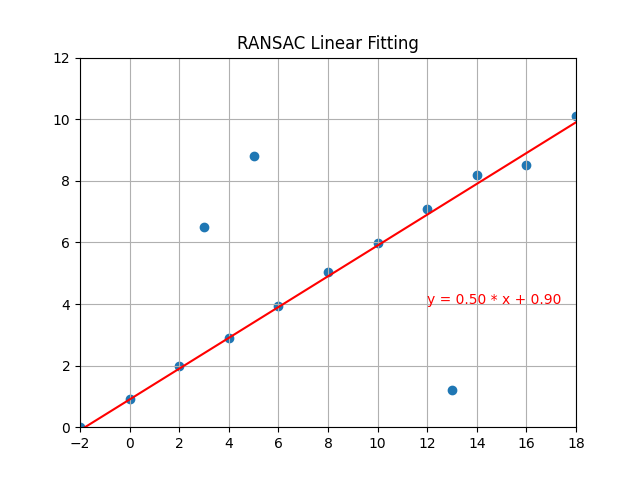
\includegraphics[width=0.8\textwidth]{../code/Q4/src/result/output.png}
        \label{fig:Q4}
    \end{figure}
\end{solution} 

\newpage

\begin{problem}
    (Programming) Get two images I1 and I2 of our campus and make sure that the 
    major parts of I1 and I2 are from the same physical plane. Stitch I1 and I2 together
    to get a panorama view using scale-normalized LoG (or DoG) based interest point
    detector and SIFT descriptors. You can use OpenCV or Matlab. You are allowed to
    call the build-in functions provided by Matlab or OpenCV.
\end{problem}

\begin{solution}

    The following are the feature point detection results of the two graphs.

    \begin{figure}[H]
        \centering
        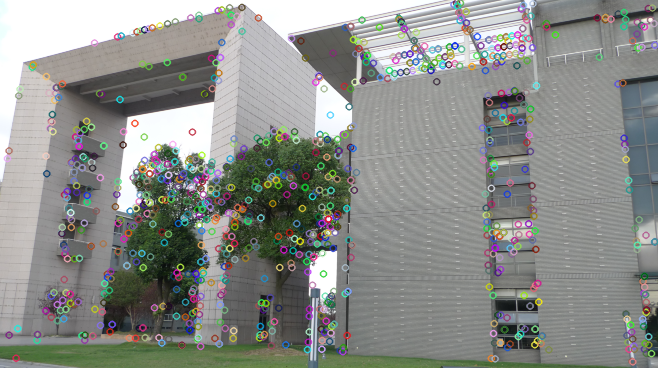
\includegraphics[width=0.8\textwidth]{../code/Q5/src/result/sse1_keypoints.png}
        \label{fig:Q5_1}
    \end{figure}

    \begin{figure}[H]
        \centering
        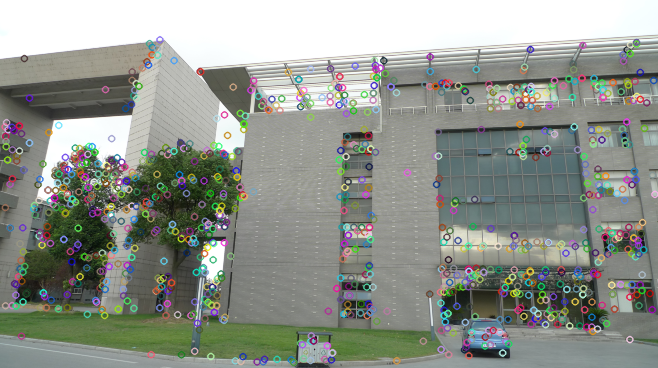
\includegraphics[width=0.8\textwidth]{../code/Q5/src/result/sse2_keypoints.png}
        \label{fig:Q5_2}
    \end{figure}

    The matching results are shown below.

    \begin{figure}[H]
        \centering
        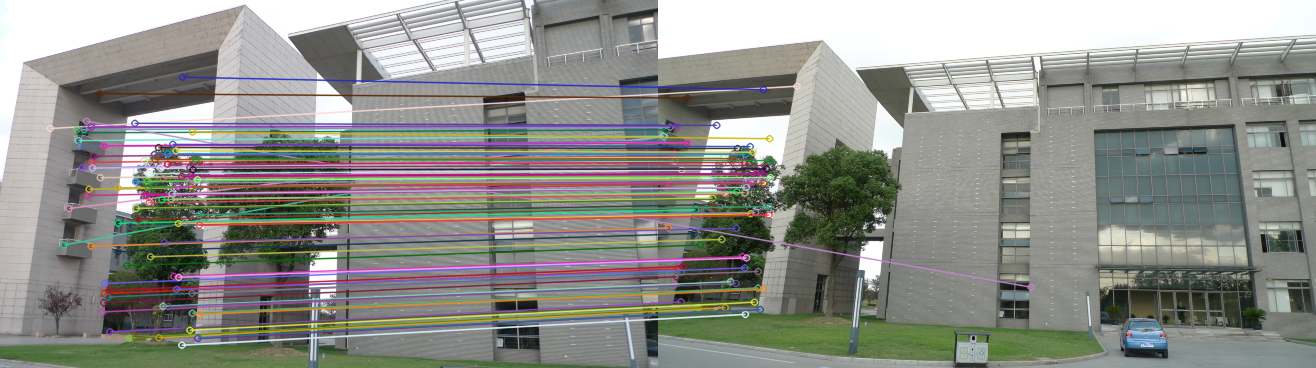
\includegraphics[width=0.8\textwidth]{../code/Q5/src/result/sse1_matches.png}
        \label{fig:Q5_3}
    \end{figure}

    The following image shows the panoramic stitching result of "the left image transformed while the right image remains unchanged."
    \begin{figure}[H]
        \centering
        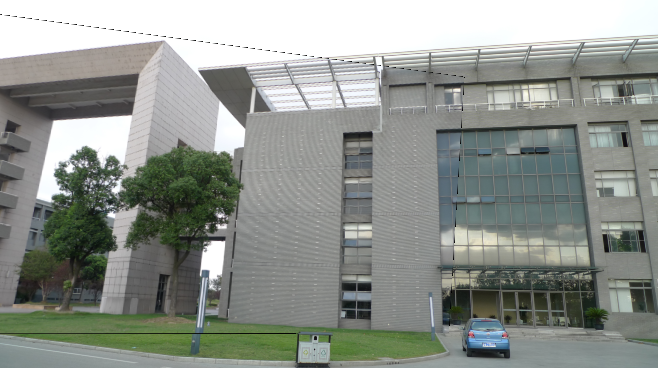
\includegraphics[width=0.8\textwidth]{../code/Q5/src/result/sse1_trans_homograyphy.png}
        \label{fig:Q5_5}
    \end{figure}

    I have also produced the result of "the left image remains unchanged while the right image is transformed," as shown in the following image.

    \begin{figure}[H]
        \centering
        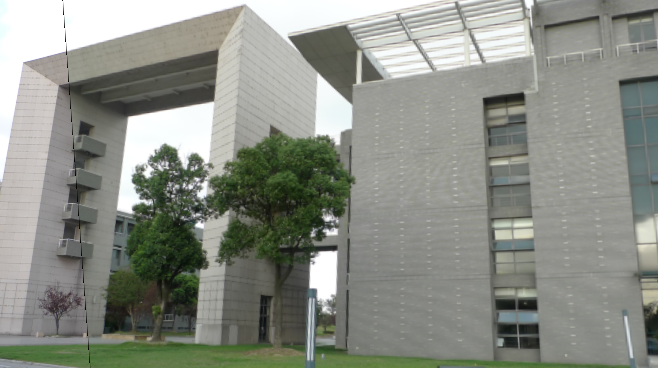
\includegraphics[width=0.8\textwidth]{../code/Q5/src/result/sse2_trans_homograyphy.png}
        \label{fig:Q5_6}
    \end{figure}
\end{solution}

\newpage

\begin{problem}
    (Programming) ORB feature point detection and matching algorithms have been
    fully implemented in the OpenCV library. Please write a C++program that invokes
    the OpenCV library’s algorithm for ORB feature point detection and matching for
    two given images, and output feature point matching results similar to the
    following given example.
\end{problem}

\begin{solution}

    The matching results are shown below.

    \begin{figure}[H]
        \centering
        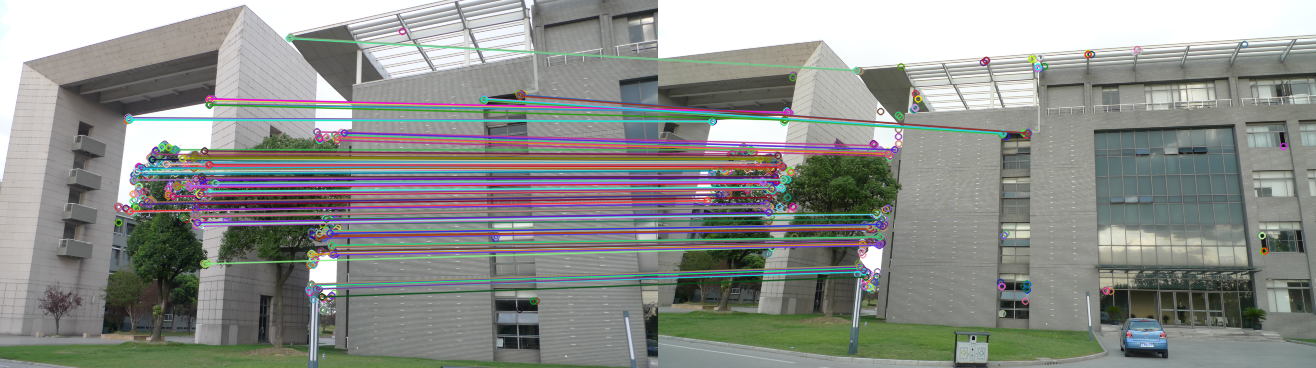
\includegraphics[width=0.8\textwidth]{../code/Q6/images/result/image_matches.png}
        \label{fig:Q6_1}
    \end{figure}

    The following image shows the panoramic stitching result of "the left image transformed while the right image remains unchanged."

    \begin{figure}[H]
        \centering
        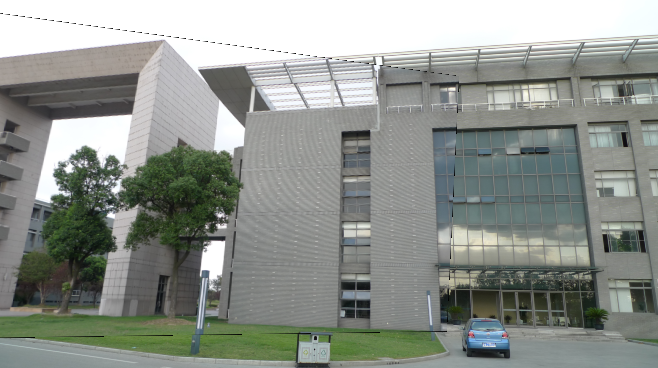
\includegraphics[width=0.8\textwidth]{../code/Q6/images/result/homograyphy.png}
        \label{fig:Q6_2}
    \end{figure}

\end{solution} 

\end{document}